\def\pgfsysdriver{pgfsys-dvipdfm.def}
%Bug in xelatex, see https://github.com/josephwright/beamer/issues/337
\documentclass[usenames,dvipsnames]{beamer}
\usepackage{tikz}
\usepackage{amsmath,amsthm,amssymb,enumerate,bbm,hyperref,mathtools,xeCJK,xpinyin,tikz-cd,stmaryrd,adjustbox,lscape,listings,changepage,epigraph,xcolor}
\usepackage[linesnumbered,ruled]{algorithm2e}
\usecolortheme{crane}

\usepackage{pgfpages}
\setbeamertemplate{note page}[plain]
\setbeameroption{show notes on second screen=right}

\usepackage{tkz-euclide,tkz-fct}

\newcommand\dhrightarrow{%
  \mathrel{\ooalign{$\rightarrow$\cr%
  $\mkern3.5mu\rightarrow$}}
}

\newcommand\dhxrightarrow[2][]{%
  \mathrel{\ooalign{$\xrightarrow[#1\mkern4mu]{#2\mkern4mu}$\cr%
  \hidewidth$\rightarrow\mkern4mu$}}
}

\newcommand\Wider[2][3em]{%
\makebox[\linewidth][c]{%
  \begin{minipage}{\dimexpr\textwidth+#1\relax}
  \raggedright#2
  \end{minipage}%
  }%
}


\theoremstyle{definition}
\newtheorem{defi}{Definition}
\newtheorem{theo}{Theorem}

\title{Elliptic curves, lattices, and some differential geometry -- part I}
\subtitle{A ``modular forms''-y gumbo}
\author{Tobias Magnusson}
\institute{Chalmers University of Technology}
\date{\today}
\subject{Mathematics}
\begin{document}
\begin{frame}[plain]
\titlepage
\end{frame}

\begin{frame}
  \frametitle{Introduction}
  \begin{itemize}
    \item Modular forms should be viewed geometrically.\pause
    \item Why?\pause
      \begin{itemize}
        \item When doing computations -- want to reduce Fourier coefficients modulo $p$.\pause~Need to make sense of modular form with different field of coefficients.\pause
        \item The geometric point of view has much richer theory.\pause
      \end{itemize}
    \item Goal of these talks:\pause~go from analytic/computational understanding to geometric understanding.
  \end{itemize}
\end{frame}

\begin{frame}
  \frametitle{What even is a modular form?}
  \begin{itemize}
    \item Function on the upper-half plane $\mathbb{H}$ that is {\bf very} symmetric.\pause
    \item Defined in terms of two actions by\pause
      \[\mathrm{SL}_2(\mathbb{Z})=\{(a,b;c,d):a,b,c,d\in\mathbb{Z},ad-bc=1\}.\]
  \end{itemize}
\end{frame}

\begin{frame}
  \frametitle{First action}
  \begin{defi}[Möbius action]
    Let $\tau\in\mathbb{H}$ and $\gamma=(a,b;c,d)\in\mathrm{SL}_2(\mathbb{Z})$. Define\pause
    \[\gamma.\tau=\frac{a\tau+b}{c\tau+d}.\]\pause
  \end{defi}
  Is left action.
\end{frame}

\begin{frame}
  \frametitle{Second action}
  \begin{defi}[Slash action]
    Let $k$ be an integer.\pause~For function $f:\mathbb{H}\to\mathbb{C}$ and $\gamma=(a,b;c,d)\in\mathrm{SL}_2(\mathbb{Z})$, define\pause
    \[(f|_k\gamma)(\tau)=(c\tau+d)^{-k}f(\gamma.\tau).\]\pause
  \end{defi}
  Is right action.
\end{frame}

\begin{frame}
  \frametitle{Modular forms of level 1}
  \begin{defi}
    Let $k$ be an integer.\pause~Then a modular form of level $1$ of weight $k$ is a function $f:\mathbb{H}\to\mathbb{C}$ such that\pause
    \begin{enumerate}[(i)]
      \item $f$ is holomorphic on $\mathbb{H}$\pause
      \item $f|_k\gamma=f$ for every $\gamma\in\mathrm{SL}_2(\mathbb{Z})$\pause
      \item $f(\tau)$ is bounded as $\tau\to i\infty$.\pause
    \end{enumerate}
  \end{defi}
  Set of modular forms of weight $k$ and level $1$ is a vector space, denoted by $M_k(\mathrm{SL}_2(\mathbb{Z}))$.
\end{frame}

\begin{frame}
  \frametitle{Examples}
  \begin{itemize}
    \item In level 1: only need to worry about Eisenstein series.\pause
    \item Let $T=(1,1;0,1)$ and let $\Gamma_\infty=\langle T,-I\rangle$. Then we define\pause
      \[E_k(\tau)=\sum_{[\gamma]\in\Gamma_\infty\backslash\mathrm{SL}_2(\mathbb{Z})}1|_k\gamma,\]\pause
    \item Converges absolutely and locally uniformly on $\mathbb{H}$, so is holomorphic and can move in slash action.\pause
    \item This reorders factors, so is the same.\pause
    \item Conclusion: $E_k(\tau)\in M_k(\mathrm{SL}_2(\mathbb{Z}))$.\pause
    \item In fact\pause
      \[\{E_4^aE_6^b:a,b\in\mathbb{Z}_{\geq 0}\text{ and }4a+6b=k\},\]\pause
      basis for $M_k(\mathrm{SL}_2(\mathbb{Z}))$.
  \end{itemize}
\end{frame}

\begin{frame}
  \frametitle{Lattices}
  \begin{itemize}
    \item Using lattices, can get ``simpler'' alternative definition of modular forms.\pause
    \item Let $\omega_1,\omega_2\in\mathbb{C}\setminus\{0\}$ not on the same line.\pause~Lattice $L$ generated by $(\omega_1,\omega_2)$ is\pause
      \[L=\mathbb{Z}\omega_1+\mathbb{Z}\omega_2.\]\pause
    \item Consider quotient $\mathbb{C}/L=\{\tau+L:\tau\in\mathbb{C}\}$.\pause
    \item $\tau+L$ has unique representative in ``fundamental parallelogram''.\pause
  \end{itemize}
  We denote the set of lattices in $\mathbb{C}$ by $\mathcal{L}(\mathbb{C})$.
\end{frame}

\begin{frame}
  \frametitle{}
  \begin{figure}[h]
    \centering
    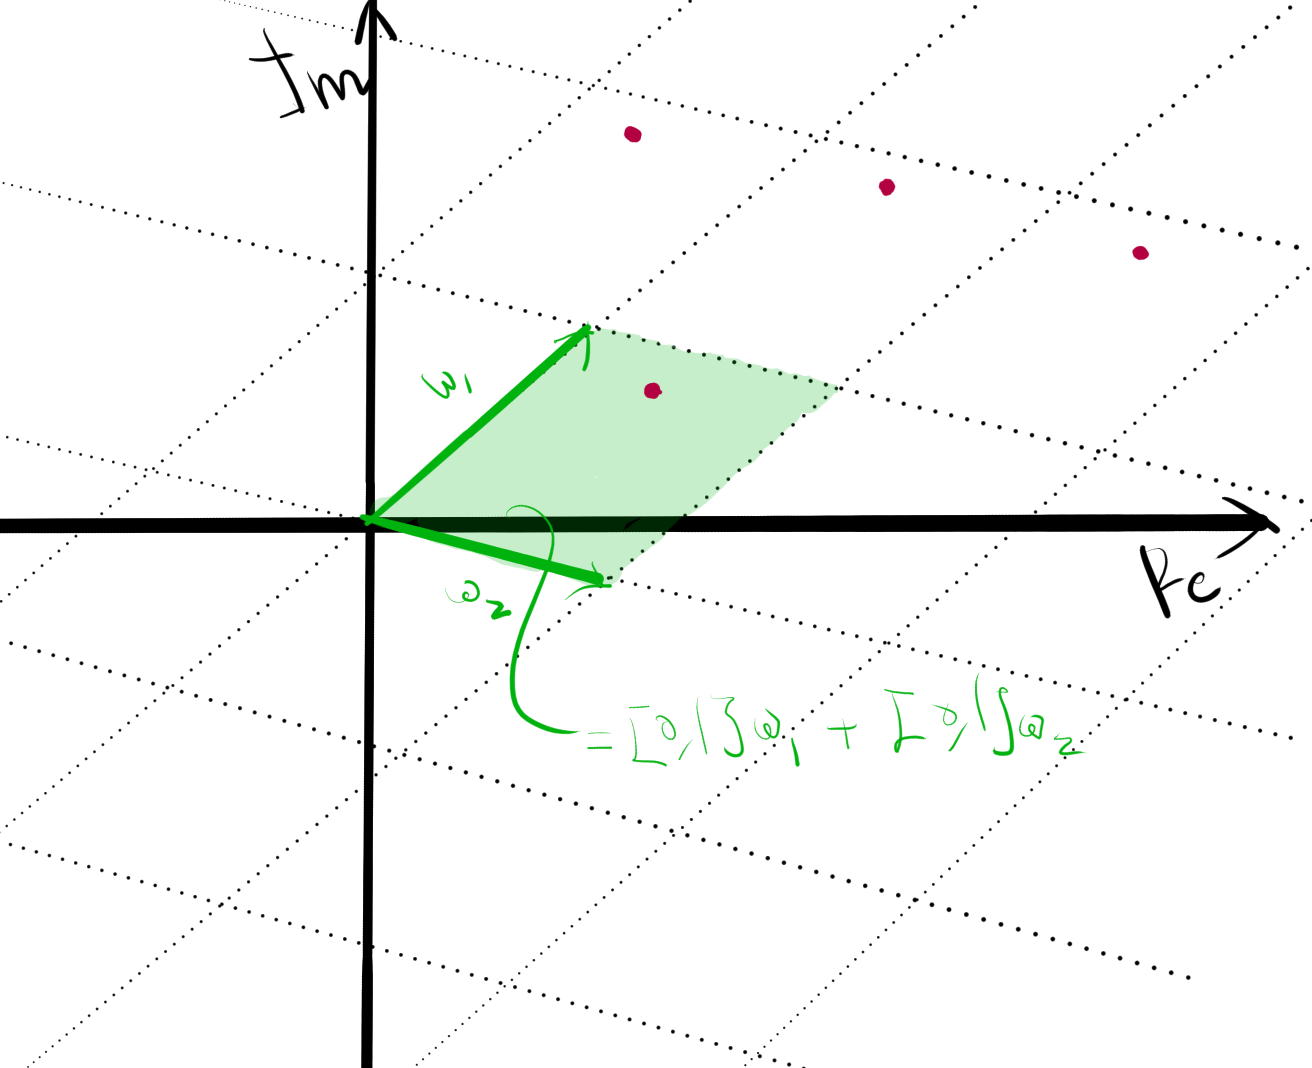
\includegraphics[width=0.9\textwidth]{lattice.png}
  \end{figure}
\end{frame}

\begin{frame}
  \frametitle{Topology}
  \begin{itemize}
    \item Homeomorphic to square with sides identified.\pause
    \item That is, homeomorphic to torus $S^1\times S^1$.
  \end{itemize}
\end{frame}

\begin{frame}
  \frametitle{Modular forms, lattice based definition}
  \begin{defi}
    Let $k$ be an integer.\pause~Then a modular form of weight $k$ is function $F:\mathcal{L}(\mathbb{C})\to\mathbb{C}$ satisfying\pause
    \begin{enumerate}[(i)]
      \item For $a\in\mathbb{C}$ fixed, define the mapping\pause
        \[L(z)=\mathbb{Z}a+\mathbb{Z}z\in\mathcal{L}(\mathbb{C}).\]\pause
        Then $F\circ L(z)$ holomorphic in $z$.\pause
      \item If $\lambda\in\mathbb{C}\setminus\{0\}$ and $L\in\mathcal{L}(\mathbb{C})$, then\pause
        \[F(\lambda L)=\lambda^{-k}F(L).\]\pause
      \item $F(\mathbb{Z}+\mathbb{Z}\tau)$ is bounded as $\tau\to i\infty$.
    \end{enumerate}
  \end{defi}
\end{frame}

\begin{frame}
  \frametitle{Equivalence}
  Can show is equivalent to previous definition by\pause
  \[f(\tau)=F(\mathbb{Z}+\mathbb{Z}\tau),\]\pause
  and\pause
  \[F(\mathbb{Z}\omega_1+\mathbb{Z}\omega_2)=\omega_2^{-k}f(\omega_1/\omega_2),\]
  for $\mathrm{Im}(\omega_1/\omega_2)>0$.
\end{frame}

\begin{frame}
  \frametitle{Weierstraß $\wp$-function}
  \begin{itemize}
    \item Allows us to associate elliptic curve to $\mathbb{C}/L$.\pause
    \item Let $z\in\mathbb{C}$ and $L\in\mathcal{L}(\mathbb{C})$. Then\pause
      \[\wp(z;L)=\frac{1}{z^2}+\sum_{l\in L\setminus\{0\}}\Big(\frac{1}{(z-l)^2}-\frac{1}{l^2}\Big).\]\pause
    \item $\wp(z;L)$ is $L$-periodic.\pause
    \item Can show:\pause~$\wp(z;L)$ meromorphic with poles only at $z\in L$.\pause
    \item $\wp'(z;L)=\sum_{l\in L}\frac{-2}{(z-l)^3}$, also $L$-periodic, poles only at $z\in L$.\pause
    \item Laurent expansion at $z=0$:\pause
      \[\wp(z)=z^{-2}+\frac{g_4}{20}z^2+\frac{g_6}{28}z^4+O(z^6),\]\pause
      where $g_4=\frac{4}{3}\pi^4E_4$ and $g_6=\frac{8}{27}\pi^6E_6$.
  \end{itemize}
\end{frame}

\begin{frame}
  \frametitle{$\wp$-function, differential equation}
  \begin{itemize}
    \item Clever usage of Liouville's theorem:\pause~bounded entire function is constant.\pause
    \item Let $E(z;L)=4\wp(z;L)^3-g_4\wp(z;L)-g_6-\wp'(z;L)^2$.\pause
    \item Using Laurent: $\lim_{z\to 0}E(z;L)=0$.\pause
    \item Since $E(z;L)$ is $L$-periodic:\pause~no poles at lattice points.\pause
    \item Hence $E(z;L)$ no poles at all,\pause~i. e. entire.\pause
    \item Fundamental parallelogram is compact,\pause~so $E(z;L)$ attains finite max there.\pause
    \item Since $L$-periodic,\pause~$E(z;L)$ bounded everywhere.\pause
    \item Liouville: $E(z;L)=E(L)$ constant,\pause~so
      \[E(L)=\lim_{z\to 0}E(z;L)=0.\]
  \end{itemize}
\end{frame}

\begin{frame}
  \frametitle{Mapping tori to elliptic curves}
  \begin{itemize}
    \item Define $\psi:\mathbb{C}/L\to\mathbb{C}^2$ by\pause
      \[\psi(z+L)=(x=\wp(z;L),y=\wp'(z;L)).\]\pause
    \item Then $y^2=4x^3-g_4x-g_6$ is elliptic curve.
  \end{itemize}
\end{frame}

\begin{frame}
  \frametitle{Can go back -- lattice of periods}
  \begin{itemize}
    \item Next talk!\pause
    \item Key: need to associate a differential form to elliptic curve.\pause
    \item Can map $(E,\omega)\mapsto L\in\mathcal{L}(\mathbb{C})$.
  \end{itemize}
\end{frame}

\begin{frame}
  \frametitle{Katz' idea}
  \begin{itemize}
    \item We know:\pause~can define modular forms on lattices.\pause
    \item Hence: try to define modular forms on elliptic curves.\pause
    \item How to ``see'' weight?\pause~Consider pairs $(E,\omega)$ with $E$ elliptic curve and $\omega$ ``differential form'' on $E$.\pause
    \item Modular form:\pause~rule $\mathbb{F}$ that assigns to $(E,\omega)$ a complex number, and that satisfies\pause
      \[\mathbb{F}(E,\lambda\omega)=\lambda^{-k}\mathbb{F}(E,\omega),\]\pause
      for $\lambda\in\mathbb{C}\setminus\{0\}$.\pause
    \item Connection: $\mathbb{F}(E,\omega)=F(L(E,\omega))$.
  \end{itemize}
\end{frame}

\begin{frame}
  \frametitle{Excerpt from ``$p$-adic Properties [...]''}
  \begin{figure}[h]
    \centering
    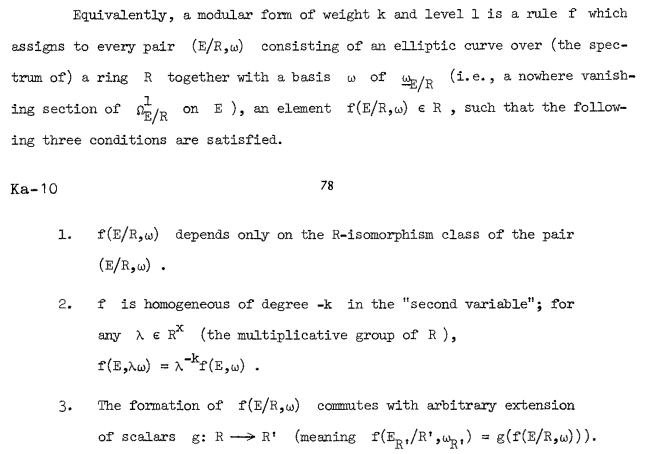
\includegraphics[width=0.8\textwidth]{excerpt.png}
  \end{figure}
  \note{Notice in particular that we now can work over other ground fields. Indeed, we can even work over rings!}
\end{frame}

\begin{frame}
  \frametitle{This talk}
  \begin{itemize}
    \item Goal: try to understand $\mathbb{C}/L$ as a complex manifold,\pause
    \item and make sense of $\omega=dz$ as a differential form.
  \end{itemize}
\end{frame}

\begin{frame}
  \frametitle{}
  \begin{figure}[h]
    \centering
    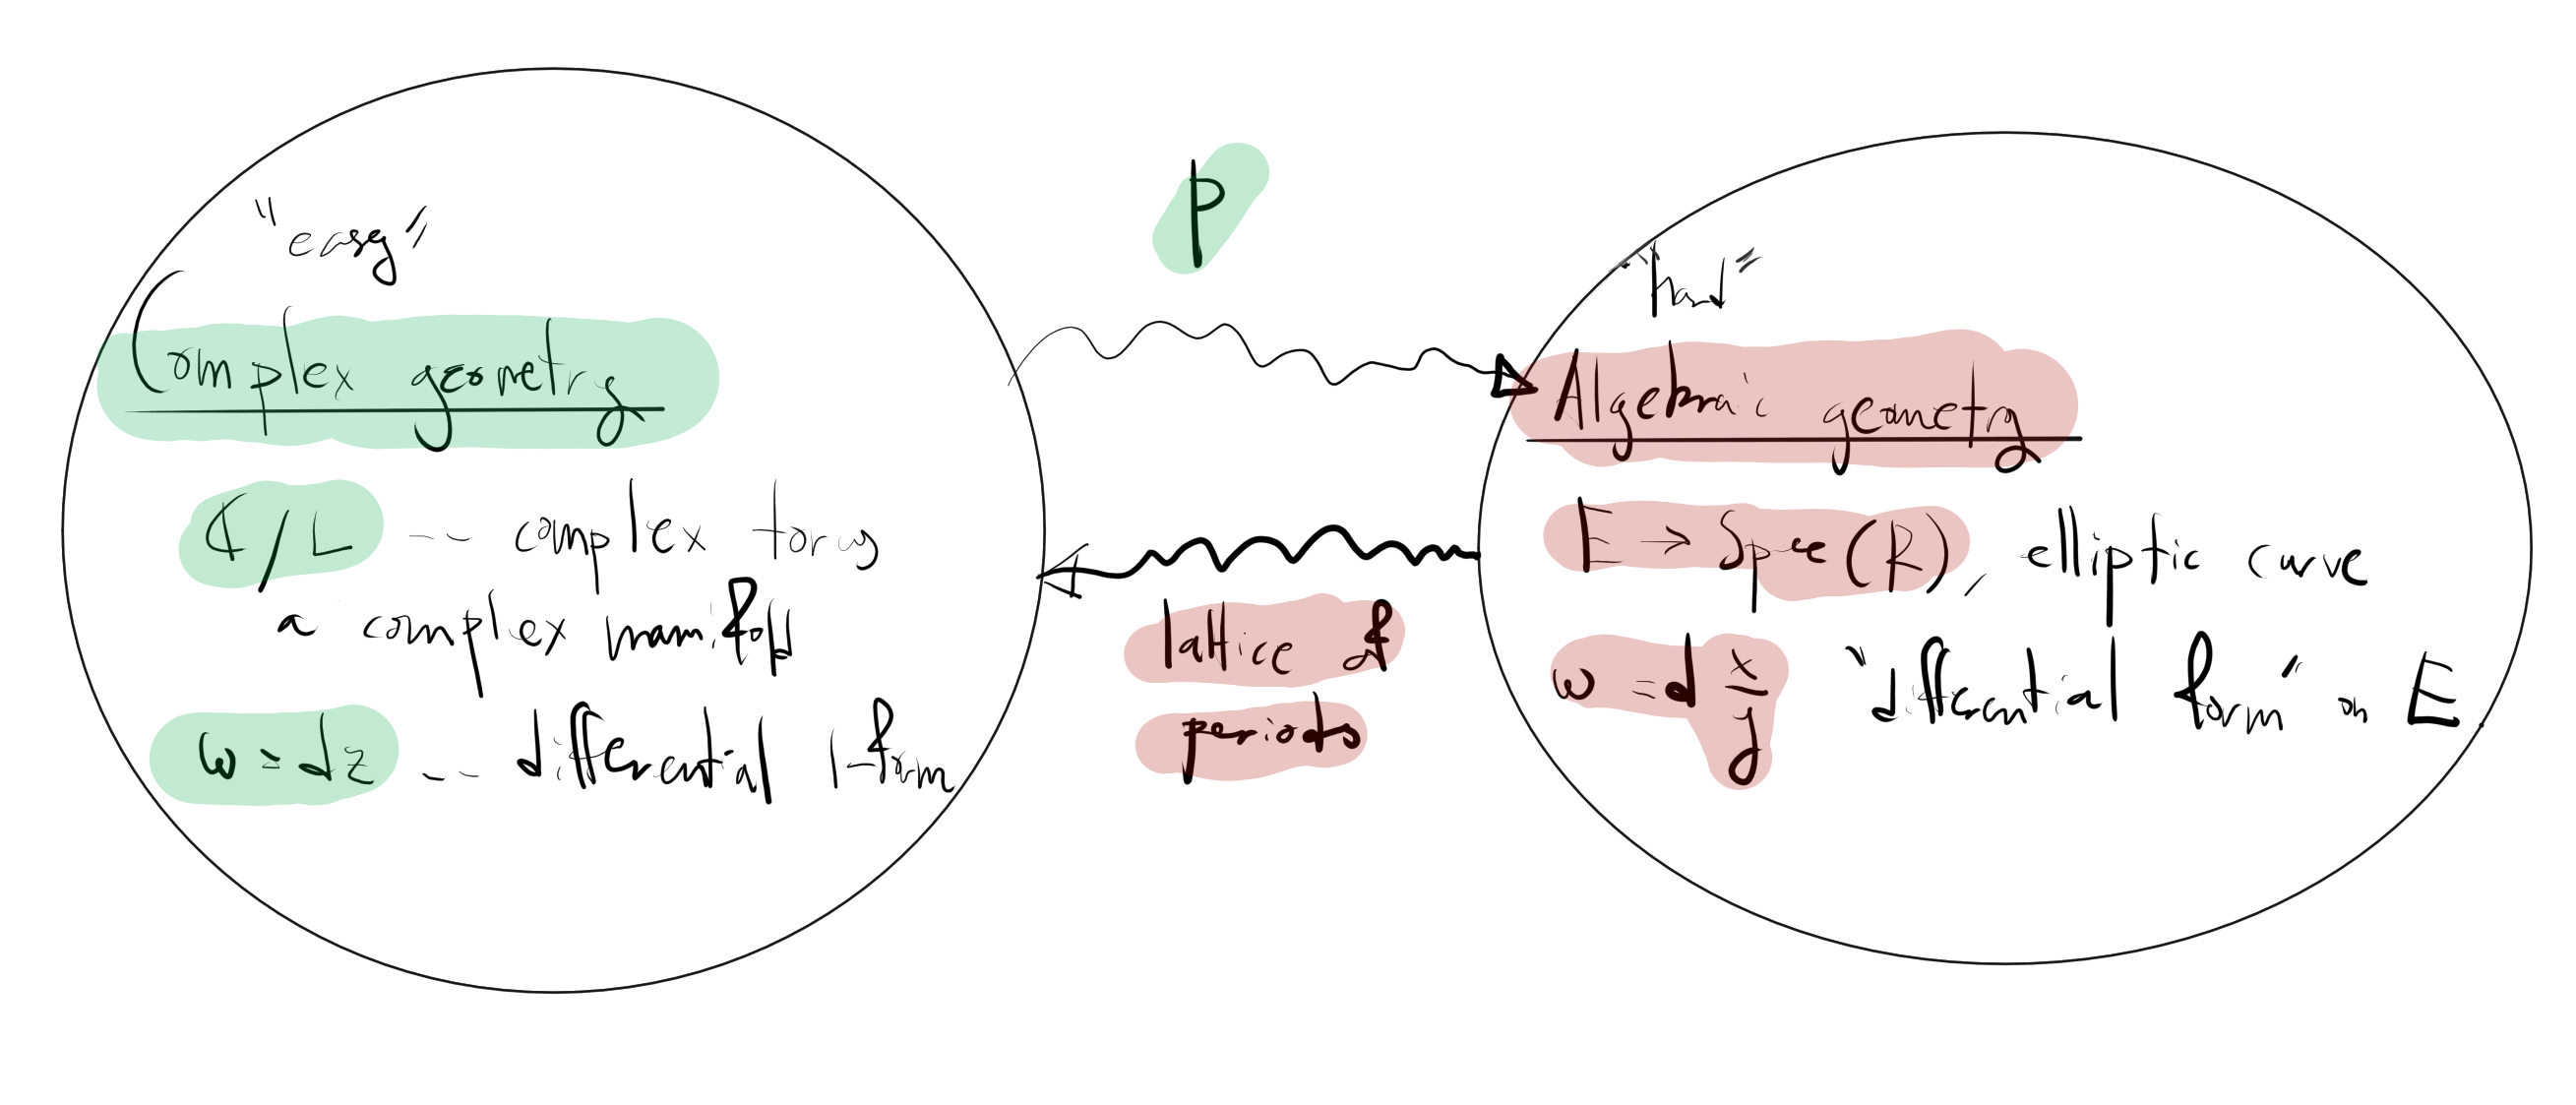
\includegraphics[width=1\textwidth]{bigpicture.png}
  \end{figure}
\end{frame}

\begin{frame}
  \frametitle{The left part}
  \begin{itemize}
    \item Complex manifolds.\pause
    \item Complex tori.\pause
    \item Differential forms.
  \end{itemize}
\end{frame}

\begin{frame}
  \frametitle{Complex coordinate system}
    Let $X$ be Hausdorff and $n\geq 1$ be an integer.\pause
    \begin{itemize}
      \item A pair $(U,\phi)$ where $U\subseteq X$ is open and $\phi:U\to B\subseteq\mathbb{C}^n$ is a homeomorphism is called a complex coordinate system in $X$.\pause
      \item If $p\in X$ is a point, then every complex coordinate system $(U\ni p,\phi)$ is called a coordinate system at $p$.\pause
      \item The components of $\phi$ are called local coordinates with respect to $(U,\phi)$,\pause
      \item and in particular the entries of $\phi(p)$ are called the coordinates of $p$ with respect to $(U,\phi)$.\pause
      \item If $f$ function in $U$, we consider it as a function of $z_1,\dots,z_n$ by
        \[(z_1,\dots,z_n)\mapsto f\circ\phi^{-1}(z_1,\dots,z_n).\]
    \end{itemize}
\end{frame}

\begin{frame}
  \frametitle{Compatible coordinate systems}
  \begin{defi}
    Let $X$ be Hausdorff and $\mathcal{U}=(U,\phi)$ and $\mathcal{V}=(V,\psi)$ be two $n$-dimensional complex coordinate systems in $X$.\pause~Then $\mathcal{U}$ and $\mathcal{V}$ are called compatible iff $U\cap V=\emptyset$, or if\pause
    \[\phi\circ\psi^{-1}:\psi(U\cap V)\to \phi(U\cap V),\]\pause
    is biholomorphic (i. e. bijective holomorphic with holomorphic inverse).
  \end{defi}
\end{frame}

\begin{frame}
  \frametitle{Atlas}
  \begin{defi}
    Let $X$ be Hausdorff and $n\geq 1$ be an integer.\pause~Then a covering (with respect to the first component) of $X$ by pairwise compatible $n$-dimensional complex coordinate systems is called an $n$-dimensional atlas on $X$.\pause

    Two atlases $\mathcal{A}_1,\mathcal{A}_2$ are called equivalent\pause~iff there exists coordinate systems $\mathcal{U}\in\mathcal{A}_1$ and $\mathcal{V}\in\mathcal{A}_2$\pause~such that $\mathcal{U}$ and $\mathcal{V}$ are compatible.\pause~We then write $\mathcal{A}_1\sim\mathcal{A}_2$.
  \end{defi}
\end{frame}

\begin{frame}
  \frametitle{Complex structure}
  \begin{defi}
    Let $X$ be Hausdorff and $n\geq 1$ be an integer.\pause~If $\mathcal{A}$ is an $n$-dimensional atlas on $X$,\pause~then an equivalence class $[\mathcal{A}]_{\sim}$ is called an $n$-dimensional complex structure on $X$.
  \end{defi}
\end{frame}

\begin{frame}
  \frametitle{Complex manifold}
  \begin{defi}
    Let $n\geq 1$ be an integer.\pause~Then an $n$-dimensional complex manifold\pause~is a second countable Hausdorff space equipped with an $n$-dimensional complex structure.
  \end{defi}
\end{frame}

\begin{frame}
  \frametitle{Trivial example}
    \begin{itemize}
      \item $\mathbb{C}^n$ is second countable Hausdorff with respect to the Euclidean topology.\pause
      \item Let\pause
        \[\mathcal{A}=\{(\mathbb{C}^n,\mathrm{id})\}.\]\pause
        Then $\mathcal{A}$ is an atlas.\pause
      \item So $[\mathcal{A}]_{\sim}$ is a complex structure.\pause
      \item Hence $(\mathbb{C}^n,[\mathcal{A}]_{\sim})$ is a complex $n$-dimensional manifold.
    \end{itemize}
\end{frame}

\begin{frame}
  \frametitle{Submanifold}
  \begin{itemize}
    \item Let $(X,[\mathcal{A}]_{\sim})$ be an $n$-dimensional complex manifold.\pause
    \item Let $B\subseteq X$ open.\pause
    \item Define $\mathcal{B}=\{(U\cap B,\phi|_{U\cap B}):(U,\phi)\in\mathcal{A}\}$.\pause~Atlas on $B$.\pause
    \item $(B,[\mathcal{B}]_{\sim})$ is $n$-dimensional complex manifold.
  \end{itemize}
\end{frame}

%\begin{frame}
%  \frametitle{Prerequisites for quotient manifolds}
%  To put complex structure on $X/{\sim}$, need:\pause
%  \begin{itemize}
%    \item Holomorphic functions on manifolds.\pause
%    \item Holomorphic maps between manifolds.\pause
%    \item Local Jacobian.\pause
%    \item Rank of a holomorphic map.\pause
%  \end{itemize}
%  Cursory.
%\end{frame}
%
%\begin{frame}
%  \frametitle{Prerequisites for quotient manifolds}
%  Let $X$ and $Y$ complex manifolds.
%  \begin{itemize}
%    \item Let $B\subseteq\mathbb{C}^n$ open. A map $\mathbf{f}=(f_1,\dots,f_m):B\to\mathbb{C}^m$ is called holomorphic if all $f_i$ are.\pause
%    \item Let $B\subseteq X$ open.\pause~A function $f:B\to\mathbb{C}$ is called holomorphic if for each $p\in B$ there is a coordinate system $(U\ni p,\phi)$ such that\pause
%      \[f\circ\phi^{-1}:\phi(U\cap B)\to\mathbb{C},\]\pause
%      is holomorphic.
%    \item Let $F:X\to Y$ be continuous.\pause~Then $F$ is called holomorphic if for any $p\in X$ there is a coordinate system $(U\ni p,\phi)$ on $X$ and $(V\ni F(p),\psi)$ with $F(U)\subseteq V$ such that\pause
%      \[\psi\circ F\circ\phi^{-1}:\phi(U)\to \psi(V),\]\pause
%      is a holomorphic map.
%  \end{itemize}
%\end{frame}
%
%\begin{frame}
%  \frametitle{Local Jacobian}
%  Let $X$ be $n$-dimensional manifold.\pause
%  \begin{itemize}
%    \item Let $f_1,\dots,f_m$ be $\mathbb{C}$-valued holomorphic defined on open $U\subseteq X$.\pause~Let $p\in U$ and $(V\ni p,\psi)$ coordinate system.\pause~Then $\mathbf{f}=(f_1,\dots,f_m):U\to\mathbb{C}^m$ and we define\pause
%      \[J_\mathbf{f}(p;\psi)=\Big(\frac{\partial(f_i\circ\psi^{-1})}{\partial z_j}(\psi(p))\Big)_{\substack{1\leq i\leq m\\1\leq j\leq n}}.\]\pause
%    \item If $(W\ni p,\phi)$ another coordinate system at $p$.\pause~Then for some invertible $n\times n$ matrix $\lambda$ it holds that\pause
%      \[J_\mathbf{f}(p;\psi)=J_\mathbf{f}(p;\phi)\cdot\lambda.\]
%  \end{itemize}
%\end{frame}
%
%\begin{frame}
%  \frametitle{Rank}
%    So $\mathrm{rk}\,J_\mathbf{f}(p;\psi)$ independent of coordinate system, define\pause
%    \[\mathrm{rk}_p(f_1,\dots,f_m)=\mathrm{rk}\,J_\mathbf{f}(p;\phi).\]
%\end{frame}
%
%\begin{frame}
%  \frametitle{Quotient manifold}
%  Let $X$ be a complex manifold of dimension $n$,\pause~let $\sim$ be an equivalence relation on $X$,\pause~and let $\pi:X\to X/{\sim}$ be $\pi(x)=[x]_{\sim}$.\pause
%  \begin{theo}
%  Suppose that:\pause
%  \begin{enumerate}[(i)]
%    \item With the quotient topology, $X/{\sim}$ is Hausdorff.\pause
%    \item For any $x_0\in X$ there exists open neighborhood $\hat{U}$ with $\pi^{-1}(\pi(\hat{U}))=\hat{U}$ of $[x_0]$ in $X$\pause~and a holomorphic map $\mathbf{f}:\hat{U}\to\mathbb{C}^{n-d}$ such that\pause
%      \begin{enumerate}[(a)]
%        \item such that $\mathbf{f}^{-1}(\mathbf{f}(x))=[x]$ for all $x\in\hat{U}$.\pause
%        \item $\mathrm{rk}_x(\mathbf{f})=n-d$ for $x\in\hat{U}$.\pause
%      \end{enumerate}
%  \end{enumerate}
%  Then $X/{\sim}$ carries the structure of an $n-d$ dimensional complex manifold such that $\pi:X\to X/{\sim}$ is a holomorphic map.\pause
%\end{theo}
%  Next: We describe the complex structure in the special case of $\mathbb{C}^n/\sum_{i=1}^n\mathbb{Z}\omega_i$ with $\{\omega_1,\dots,\omega_n\}$ real-linearly independent.
%\end{frame}
%
%Define neighborhoods, show are saturated, and define f.
%Go to theorem to show how complex structure looks like.
\begin{frame}
  \frametitle{Complex tori}
  \begin{itemize}
    \item Let $L=\sum_{i=1}^n\mathbb{Z}\omega_i$ and let $L$ act on $\mathbb{C}^n$ by translation.\pause
    \item Consider $\mathbb{C}^n/L$,\pause~let $\pi:\mathbb{C}^n\to\mathbb{C}^n/L$ by $\pi(z)=z+L$.\pause
    \item For $U\subset\mathbb{C}^n$ open have\pause
      \[\pi^{-1}(\pi(U))=\bigcup_{\lambda\in L}U+\lambda,\]\pause
      so $\pi(U)$ open.\pause
    \item Let $\tilde{x}\in\mathbb{C}^n/L$ and take $x\in\mathbb{C}^n$ such that $\pi(x)=\tilde{x}$.\pause~Let $U\ni x$ open, satisfying\pause
      \[\pi|_U:U\to\pi(U),\]\pause
      bijective (Careful!).\pause~Then because continuous open bijective, is homeomorphism.\pause
    \item Define coordinate system at $\tilde{x}$ by $(\pi(U),\phi)$ where $\phi=\pi|_U^{-1}:\pi(U)\to U$.\pause
    \item Does it make an atlas?
  \end{itemize}
\end{frame}

\begin{frame}
  \frametitle{Is it an atlas?}
  \begin{itemize}
    \item Since can form for any $\tilde{x}\in\mathbb{C}^n/L$, it must be is cover.\pause
    \item Suppose $(\pi(U),\pi|_U^{-1})$ and $(\pi(V),\pi|_V^{-1})$ satisfies\pause
      \[\pi(U)\cap\pi(V)=\pi(U\cap V)\neq\emptyset.\]\pause
    \item Then\pause
      \[\pi|_V^{-1}(\pi(U\cap V))=U\cap V\text{ and }\pi|_U^{-1}(\pi(U\cap V))=U\cap V.\]\pause
    \item If $a\in U\cap V$, then
      \[\pi|_U^{-1}\circ\pi|_V(a)=\pi|_U^{-1}(\pi(a))=a,\]\pause
      so $\pi|_U^{-1}\circ\pi|_V=\mathrm{id}$.\pause
    \item Clearly biholomorphic.
  \end{itemize}
\end{frame}

\begin{frame}
  \frametitle{$\pi$ locally bijective and $\mathbb{C}^n/L$ Hausdorff}
  Follows from:
  \begin{itemize}
    \item Bijective:\pause~if $z\in\mathbb{C}^n$, there exists $U\ni z$ open such that $(U+\lambda)\cap U=\emptyset$ unless $\lambda=0$.\pause
    \item Take $U$ as above, say $\pi(a_1)=\pi(a_2)$ with $a_1,a_2\in U$, then\pause
      \[(U+a_1-a_2)\ni a_2+(a_1-a_2)=a_1\in U,\]\pause
      so $a_1=a_2$.\pause~Surjective immediate.\pause
    \item Hausdorff:\pause~if $\pi(z_1)\neq\pi(z_2)$ then exists opens $U\ni z_1$ and $V\ni z_2$ such that
      \[(U+\lambda)\cap V=\emptyset,\]\pause
      for every $\lambda\in L$.\pause
    \item Say $[z_1]\neq [z_2]$, pick $U,V$ as above.\pause~Then if $z\in\pi(U)\cap\pi(V)$ it holds that $z=u+L=v+L$ for some $u\in U$ and $v\in V$, so\pause
      \[(U+v-u)\ni u+(v-u)=v\in V,\]\pause
      so $z$ cannot exist.\pause~Hence $\pi(U)\cap\pi(V)=\emptyset$.
  \end{itemize}
\end{frame}

\begin{frame}
  \frametitle{Conclusion}
  \begin{itemize}
    \item For proofs of these two facts, see e. g. Fritzsche and Grauert.\pause
    \item Now $\mathbb{C}^n/L$ is complex manifold.\pause
    \item What about $dz$?
  \end{itemize}
\end{frame}

\begin{frame}
  \frametitle{Derivations}
  Let $X$ be an $n$-dimensional manifold and let $a\in X$ be a point.\pause~For $B\subseteq X$ open let\pause
  \[\mathcal{E}(B,\mathbb{C})=\{f:B\to\mathbb{C}:\forall\text{ c. s. }(U,\phi)\text{ s. t. }U\cap B\neq\emptyset\text{, }f\circ\phi^{-1}\text{ is smooth}\},\]\pause
  and\pause 
  \[\mathcal{E}(B)=\{f:B\to\mathbb{R}:\forall\text{ c. s. }(U,\phi)\text{ s. t. }U\cap B\neq\emptyset\text{, }f\circ\phi^{-1}\text{ is smooth}\}.\]\pause
  \begin{defi}
    A derivation on $X$ at $a$ is an $\mathbb{R}$-linear map $v:\mathcal{E}(X)\to\mathbb{R}$ satisfying\pause
    \[v[f\cdot g]=v[f]\cdot g(a)+f(a)\cdot v[g].\]
  \end{defi}
\end{frame}

\begin{frame}
  \frametitle{Can work locally}
  \begin{itemize}
    \item Using cut-off functions, can see if $f|_U=0$ for some open neighborhood $U\ni a$,\pause~then $v[f]=0$ for every derivation on $X$ at $a$.\pause
    \item Means we can work with local coordinates.\pause
    \item Let $(U,\phi=(z_1,\dots,z_n))$ be local coordinates at $a$,\pause~write $z_k=x_k+iy_k$ and\pause
      \begin{align*}
        (\partial/\partial x_k)_a[f]&=(f\circ\phi^{-1})_{x_i}(\phi(a))\\
        (\partial/\partial y_k)_a[f]&=(f\circ\phi^{-1})_{y_i}(\phi(a))
      \end{align*}
  \end{itemize}
\end{frame}

\begin{frame}
  \frametitle{Tangent space}
  \begin{itemize}
    \item Let $\mathbb{T}_a^\mathbb{R}(X)$ be real vector space of derivations on $X$ at $a$.\pause
    \item For $f\in\mathcal{E}(X,\mathbb{C})$ write $f=g+ih$ and define $v[f]=v[g]+iv[h]$.\pause
    \item Define $J(v)[f]=iv[f]$ and $(a+ib)v=av+b\cdot J(v)$.\pause
    \item Then $T_a(X)$ is complexification $(T_a^\mathbb{R}(X)\oplus T_a^\mathbb{R}(X),J)$.\pause
  \end{itemize}
  Has real dimension $2n$ with basis:\pause
  \[\{(\partial/\partial x_1)_a,\dots,(\partial/\partial x_n)_a,(\partial/\partial y_1)_a,\dots,(\partial/\partial y_n)_a\}\]
\end{frame}

\begin{frame}
  \frametitle{$1$-forms on a complex manifold}
  Let $X$ be $n$-dimensional complex manifold and $x\in X$ a point.
  \begin{itemize}
    \item Write $T=T_x(X)$ and $T^\vee=\mathrm{Hom}_\mathbb{R}(T,\mathbb{R})$.\pause
    \item Cotangent space: $F=T^\vee\oplus iT^\vee$.\pause~Note: is of {\bf complex} dimension $2n$.\pause
    \item Let $f$ be smooth function (real- or complex-valued) on neighborhood of $x$, let:\pause
      \[(df)_x(v)=v[f],\]\pause
      for $v\in T$.\pause~Then $(df)_x\in F$.\pause~Example of a differential $1$-form on $X$.\pause
    \item Let $(U,\phi)$ coordinate system at $x$.\pause~Write\pause
      \[dz_i=(d\phi_i)_x.\]
  \end{itemize}
\end{frame}

\begin{frame}
  \frametitle{Conclusion for today}
  Now we know what
  \[(\mathbb{C}/L,dz),\]
  means!
\end{frame}

\begin{frame}
  \frametitle{Part 2}
  \begin{itemize}
    \item Explain ``lattice of periods''.\pause~Need integration.\pause
    \item Consider right part of ``big picture''.\pause~Generalize $dz$ to differential on elliptic curve (or any scheme).\pause
    \item $q$-series expansion from a geometric point of view\pause~-- the Tate curve.
  \end{itemize}
\end{frame}

\begin{frame}
  \frametitle{}
  \begin{figure}[h]
    \centering
    {\Huge\tt gg,bye}
  \end{figure}
\end{frame}
%When defining derivations, make sure to mention the basis in terms of (\partial/\partial x_i)_a and (\partial/\partial y_i)_a
%This makes it easier to think of them.
\end{document}
